\documentclass{sciposter}
\usepackage{lipsum}
\usepackage{epsfig}
\usepackage{amsmath}
\usepackage{amssymb}
\usepackage{multicol}
\usepackage{listings}
\usepackage{graphicx,url}
\usepackage[spanish, spain]{babel}   
\usepackage[utf8]{inputenc}
%\usepackage{fancybullets}
\newtheorem{Def}{Definition}


\title{Proyecto Integrador Nº0
\\ }
%Título do projeto

\author{Ignacio Nahuel Chantiri 69869/1}
%nome dos autores

\institute 
{Facultad de Ingeniería de la Universidad Nacional de La Plata}
%Nome e endereço da Instituição

%\date is unused by the current \maketitle



\begin{document}
%define conference poster is presented at (appears as footer)



\maketitle

%%% Begin of Multicols-Enviroment
\begin{multicols*}{2}

%%% Introduction
\section{Introducción}
El siguiente informe resume las características del sistema desarrollado, la justificación de la elección de sus partes, y un desglose de las distintas operaciones posibles. 

El sistema lee secuencialmente instrucciones de 8 bits almacenadas en una memoria EPROM de 4096 celdas.\\
El principal propósito es manejar hasta 2 operandos de 4 bits y realizar dos operaciones aritméticas simples, una de suma y otra de multiplicación por dos, siguiendo una secuencia de instrucciones programable.

\section{Estructura}
\subsection{Diagrama general}
El esquema simplificado del sistema se dibuja en la Figura \ref{fig:diagramageneral}:

\begin{figure}[H]
    \centering
    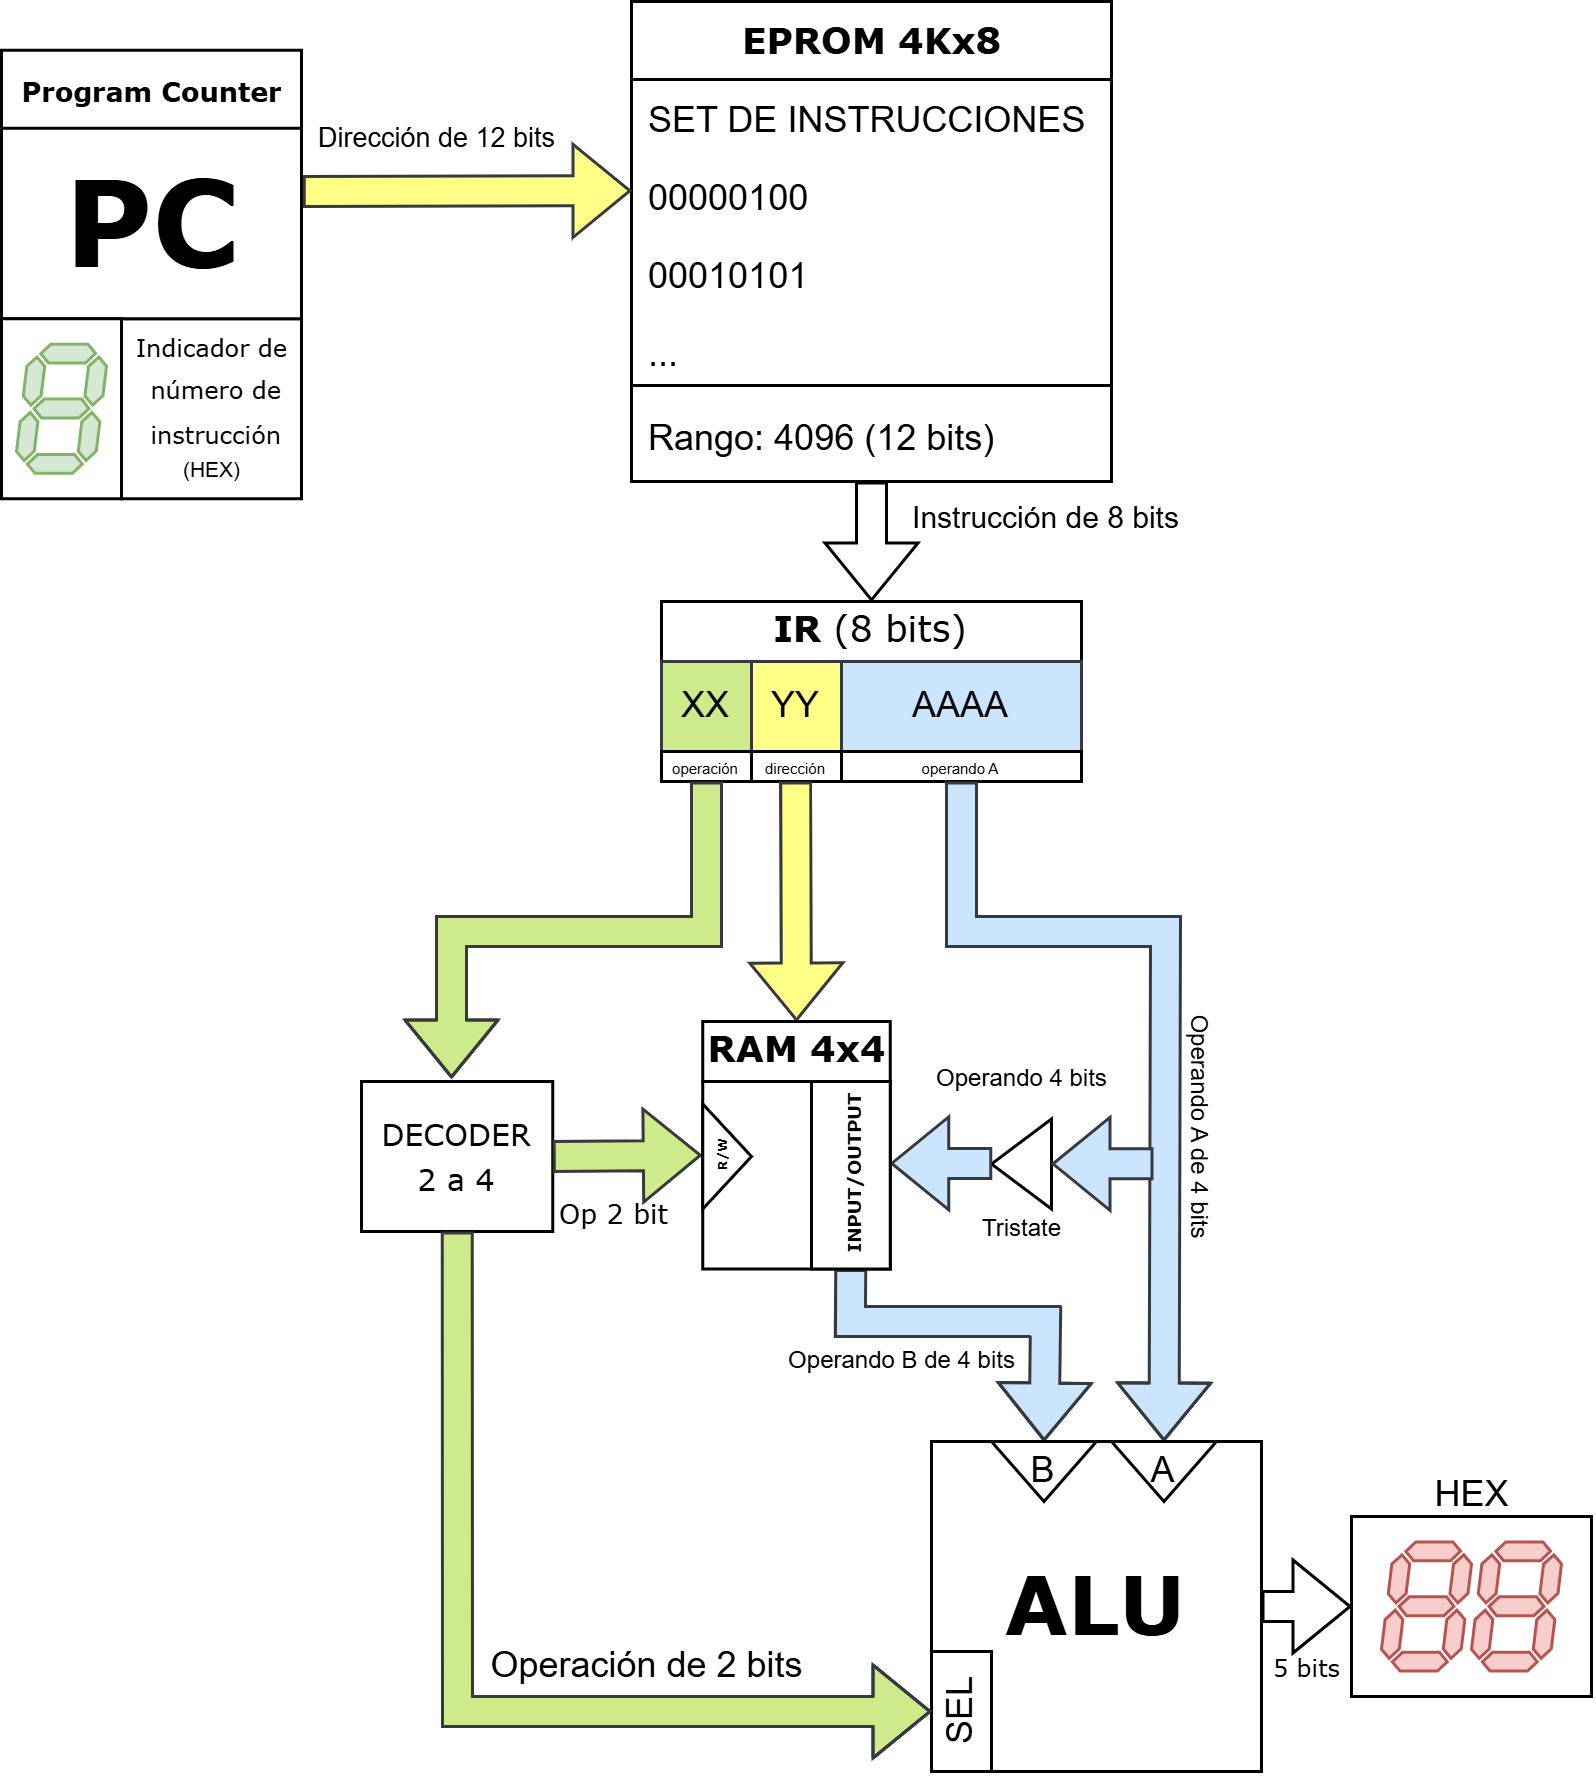
\includegraphics[width=0.7\linewidth]{Esquema general.png}
    \caption{Diagrama general del sistema implementado.}
    \label{fig:diagramageneral}
\end{figure}

En el Anexo al final de este documento se encuentra la implementación real en Proteus.

\subsection{Linea temporal}

El modo de trabajo del sistema se desarrolla durante dos ciclos del reloj. Siguiendo el esquema anterior, la linea temporal es la siguiente:

\begin{enumerate}
    \item Al primer flanco ascendente, el \textbf{PC} (Program Counter) se actualiza al valor 0000 0000.
    \item La \textbf{EPROM}, encargada de almacenar las instrucciones, recibe este valor como una dirección, y pone a su salida el contenido de la dirección 0000 0000.
    \item El \textbf{IR} (Registro 8 bits) toma este contenido en el siguiente flanco ascendente y lo interpreta como una instrucción con formato XX - YY - AAAA (8 bits). A partir de aquí, cada sección de la instrucción toma un camino distinto.
    \item La operación codificada en los dos primeros bits (XX) se decodifica en el \textbf{Decoder 2 a 4}, que indica a la \textbf{ALU} la operación aritmética que debe realizar; y a la \textbf{RAM} si debe leer, escribir o apagarse.
    \item La dirección del tercer y cuarto bit (YY) pasa a seleccionar una de las celdas de la \textbf{RAM}, que almacena un operando.
    \item Los últimos 4 bits (AAAA) son de datos, y pueden servir como operando en la \textbf{ALU}, o pueden ser guardados en la misma \textbf{RAM}, según la operación indicada.
\end{enumerate}

\section{Instrucciones}
\subsection{Formato de las instrucciones}

Las instrucciones cargadas en la EPROM son de 8 bits y cumplen con el siguiente formato:

\begin{center}
    XX - YY - AAAA
\end{center}

Donde: 

\begin{itemize}
    \item \textbf{XX:} Operación
    \item \textbf{YY:} Dirección de memoria de la RAM
    \item \textbf{AAAA:} Operando A
\end{itemize}

\subsection{Operaciones}
Las posibles operaciones del sistema se indican en la siguiente tabla:

\begin{table}[h]
    \centering
    \renewcommand{\arraystretch}{1.3} 
    \begin{tabular}{|c|c|}
        \hline
        \textbf{Código de Instrucción} & \textbf{Instrucción} \\ 
        \hline
        11 - YY - AAAA & Leer\textsuperscript{(1)} de la RAM la dirección YY \\ 
        00 - YY - AAAA & Escribir en la RAM el dato AAAA en YY \\ 
        01 - YY - AAAA & Sumar el dato de la posición YY con AAAA \\ 
        11 - YY - AAAA & Realizar la operación 2A (shift) \\ 
        \hline
    \end{tabular}
    \caption{Tabla de operaciones}
    \label{tab:operaciones}
\end{table}

\textsuperscript{(1) El dato leído se muestra en el display del operando B.}\\


\subsection{Programa}

Con el archivo .bin adjunto, se cargó en la memoria EPROM el siguiente conjunto de 14 instrucciones que el sistema recorre de manera secuencial:

\begin{table}[h]
    \centering
    \renewcommand{\arraystretch}{1.2}
    \begin{tabular}{|c|c|c|c|c|c|l|}
        \hline
        \textbf{Nº} & \textbf{OP} & \textbf{DIR} & \textbf{DATA} & \textbf{HEX} & \textbf{INSTRUCCIÓN} \\
        \hline
        0 & 00 & 00 & 0110 & 06 & ESCRIBE EL 0110 (4) EN LA DIRECCI\'ON 00 \\
        1 & 00 & 01 & 0110 & 16 & ESCRIBE EL 0110 (6) EN LA DIRECCI\'ON 01 \\
        2 & 00 & 10 & 0001 & 21 & ESCRIBE EL 0001 (1) EN LA DIRECCI\'ON 10 \\
        3 & 00 & 11 & 1111 & 3F & ESCRIBE EL 1111 (15) EN LA DIRECCI\'ON 11 \\
        4 & 11 & 00 & 0000 & C0 & LEE LO QUE HAY EN LA DIRECCI\'ON 11 (15) \\
        5 & 11 & 01 & 0000 & D0 & LEE LO QUE HAY EN LA DIRECCI\'ON 10 (1) \\
        6 & 11 & 10 & 0000 & E0 & LEE LO QUE HAY EN LA DIRECCI\'ON 01 (6) \\
        7 & 11 & 11 & 0000 & F0 & LEE LO QUE HAY EN LA DIRECCI\'ON 00 (6) \\
        8 & 01 & 00 & 0001 & 41 & SUMA LO QUE EST\'A EN LA DIRECCI\'ON 00 (6) CON 0001 (1) = 7 \\
        9 & 01 & 01 & 0010 & 52 & SUMA LO QUE EST\'A EN LA DIRECCI\'ON 01 (6) CON 0010 (2) = 8 \\
        A & 01 & 10 & 1000 & 68 & SUMA LO QUE EST\'A EN LA DIRECCI\'ON 10 (1) CON 1000 (8) = 9 \\
        B & 01 & 11 & 0001 & 71 & SUMA LO QUE EST\'A EN LA DIRECCI\'ON 11 (15) CON 0001 (1) = 16\\
        C & 10 & 00 & 0001 & 81 & TOMA EL OPERANDO A (0001)(1) Y LO MULTIPLICA POR 2 = (00010) 2 \\
        D & 10 & 00 & 1000 & 88 & TOMA EL OPERANDO A (1000)(8) Y LO MULTIPLICA POR 2 = (10000) 16 \\
        \hline
    \end{tabular}
    \caption{Set de instrucciones}
    \label{tab:instrucciones}
\end{table}

\subsection{Contenido del archivo .bin}
Las instrucciones entonces quedan escritas en hexadecimal y de manera secuencial del siguiente modo:

\begin{center}
\begin{lstlisting}
06
16
21
3F
C0
D0
E0
F0
41
52
68
71
81
88
\end{lstlisting}
\end{center}

\section{Componentes}

A continuación se detallan los componentes utilizados para cada bloque.

\subsection{Program Counter (PC)}
Es un \textbf{Contador Sincrónico} de \textbf{12 bits} compuesto por flip-flops tipo 'D'.\\
Se utilizaron 3 integrados CD4076, que contienen 4 flip-flops D cada uno. Se implementó además un bloque de lógica combinacional adecuada para conectarlos entre sí.

\subsection{Memoria EPROM de instrucciones}
Esta memoria de 32K (4Kx8) contiene el programa (4096 posibles instrucciones de 8 bits cada una).\\
Se utilizó un integrado F2732.

\subsection{Registro IR}
El registro \textbf{IR} es de una celda de 8 bits y está conformado por dos integrados CD4076 de 4 bits cada uno.
Este registro está obviamente sincronizado con el reloj, por lo que las instrucciones se actualizan con el flanco ascendente.\\
La función del \textbf{IR} es contener la instrucción actual y dividirla en secciones para su procesamiento.

\subsection{Unidad Aritmético-Lógica (ALU)}
La \textbf{ALU} implementada tiene sólo dos operaciones principales: 
\begin{itemize}
    \item Una \textbf{suma de dos operandos de 4 bits (A + B)}
    \item Un shift de una cifra a la izquierda de los bits del operando A, o \textbf{multiplicación de A por dos (2*A)}
\end{itemize}
La elección del modo se realiza con un selector de 2 bits, OP1 y OP0, y el resultado se muestra en la salida de 5 bits.\\

Por un lado, la suma se realiza con un predictor de carry de 4 bits, mientras que el shift es una simple conexión entrada-salida adecuada, sin lógica combinatoria, limitando el corrimiento de bits a solo una posición.
Además se incluyó un modo de alta impedancia de salida con tres tristate cuádruples 74125, que permite apagar un display de salida cuando no se está utilizando ninguna operación.\\
El set de operaciones posibles queda definido en la siguiente tabla:

\begin{table}[h]
    \centering
    \begin{tabular}{|c|c|c|c|}
        \hline
        \multicolumn{2}{|c|}{\textbf{Selección modo}} & \multicolumn{2}{|c|}{\textbf{Salidas activo en alto}} \\
        \hline
        \textbf{OP1} & \textbf{OP0} & \textbf{Operación} & \textbf{Descripción} \\
        \hline
        0 & 0 & Z & Salida en alta impedancia \\
        0 & 1 & A + B & Suma entre el operando A y el  \\
        1 & 0 & 2A & Multiplicación del operando A por dos (shift) \\
        1 & 1 & Z & Salida en alta impedancia \\
        \hline
    \end{tabular}
    \caption{Tabla de operaciones}
    \label{tab:operaciones}
\end{table}


\subsection{RAM 4X4}
La memoria \textbf{RAM de 4 celdas de palabras de 4 bits} está conformada por flip-flops tipo 'D' individuales (reutilizado del ejercicio de la práctica).\\
Tiene capacidad de lectura y escritura por el mismo bus de datos (IO) se accede a cada dirección de memoria con los selectores S1 y S0.

\newpage

\subsection{Decoder de operaciones}
Es un pequeño \textbf{módulo decodificador de 2 a 4 bits}.\\
Toma como entrada los primeros 2 bits de las instrucciones, y a su salida dispone dos bits hacia la \textbf{ALU} para seleccionar la operación aritmética, y otros dos hacia la \textbf{RAM} que indica lectura, escritura o apagado.\\
La lógica que permite este decoder es la siguiente:
\begin{itemize}
    \item Cuando se recibe la instrucción de \textbf{escribir}, pone el pin RW de la \textbf{RAM en modo escritura y en enable}, y \textbf{enciende el tristate} para el paso de la información a los pines IO de la RAM.
    Además selecciona el \textbf{modo alta impedancia en la ALU}.
    \item Cuando se recibe la instrucción de \textbf{leer}, pone el pin RW de la \textbf{RAM en modo lectura y en enable}, y \textbf{apaga el tristate} para cortar la llegada de información a los pines IO.
    Además selecciona el \textbf{modo alta impedancia en la ALU}.
    \item Cuando se recibe la instrucción de \textbf{sumar}, pone el pin RW de la \textbf{RAM en modo lectura} (para acceder al operando B) \textbf{y en enable}, y los selectores de 
    la \textbf{ALU en modo suma}.
    \item Cuando se recibe la instrucción de \textbf{multiplicar A por 2}, \textbf{apaga la RAM con el enable} (para apagar la pantalla del operando B y solo mostrar el A), y pone los selectores de la  \textbf{ALU en modo multiplicación}.
\end{itemize}
Se realizó con dos de las 4 compuertas OR del integrado 4071, un negador y las conexiones adecuadas.

\subsection{Tristate de 4 bits}
Se utilizó un tristate cuádruple 74125.\\
Su función es el control de datos que llegan a los IO de la \textbf{RAM}, permitiendo en un caso conectarla a un bus para su escritura, y en el otro cortar el bus para que pueda ser leída sin interferencia.

\section{Entradas y Salidas de información}

\subsection{Entradas}

Solo se cuenta con un método de entrada:

\begin{itemize}
    \item BOTÓN SIGUIENTE INSTRUCCIÓN: Es el botón que se encuentra al lado del display que indica el número de instrucción. Al presionarlo, el sistema continúa a la siguiente instrucción.
\end{itemize}

\subsection{Salidas}

La información se accede mediante displays y leds:

\begin{itemize}
    \item DISPLAY 7 SEGMENTOS OPERANDO A: Muestra el dato de 4 bits del operando A en formato hexadecimal.
    \item DISPLAY 7 SEGMENTOS OPERANDO B: Muestra el dato de 4 bits del operando B en formato hexadecimal. La operación de lectura muestra el dato leído a través de este mismo display.
    \item DOBLE DISPLAY 7 SEGMENTOS RESULTADO: Solo se enciende cuando la ALU se utiliza alguna de las operaciones aritméticas. Muestra el resultado de 5 bits en formato hexadecimal.
    \item DISPLAY NÚMERO DE LÍNEA DE INSTRUCCION: Muestra la instrucción actual, en formato hexadecimal.
    \item LEDS INDICADOR DE OPERACIÓN: El led encendido indica la operación actual. R = READ, W = WRITE, + = SUMA, X = MULTIPLICACIÓN.
\end{itemize}

\end{multicols*}

\newpage

\section{Anexo: Implementación en Proteus}

A continuación se muestra el diagrama final implementado en Proteus junto con el tablero de control.

\begin{figure}[H]
    \centering
    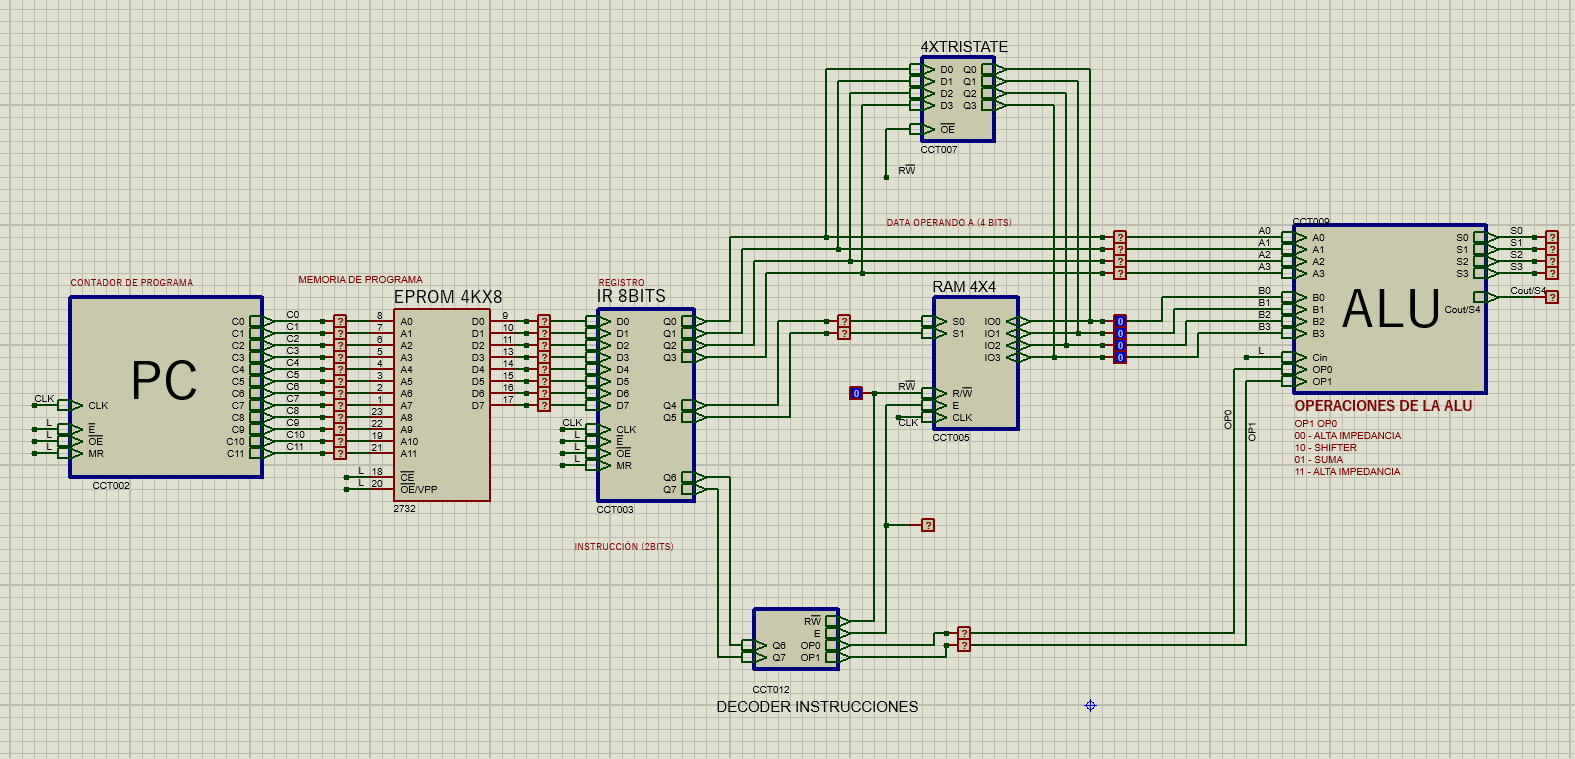
\includegraphics[width=1\linewidth]{Implementacion en proteus.png}
    \caption{Implementación del sistema en Proteus}
    \label{fig:implementacion}
\end{figure}

\begin{figure}[H]
    \centering
    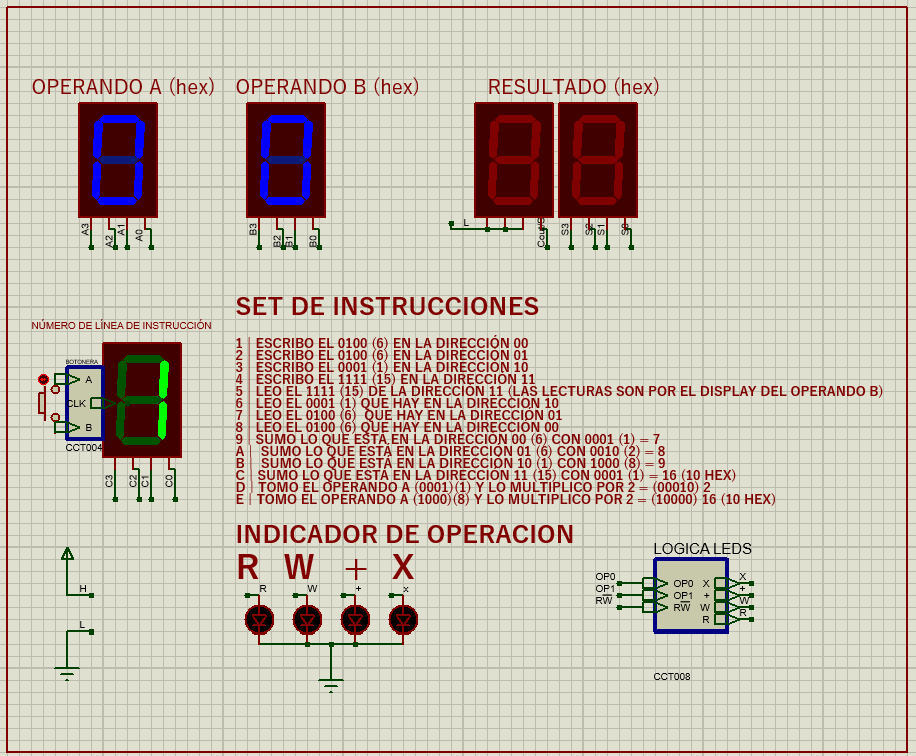
\includegraphics[width=0.7\linewidth]{Tablero de control.png}
    \caption{Tablero de control}
    \label{fig:tabcontrol}
\end{figure}

\end{document}